% chapters/09-growth-scaling.tex

\chapter{Growth and Scaling Strategies}

\begin{importantbox}
This chapter provides frameworks and strategies for scaling your Nigerian business operations, with specific guidance for different business types and regions.
\end{importantbox}

\FloatBarrier
\section{Market Expansion Framework}

\subsection{Growth Model Selection}
\begin{figure}[htbp]
    \centering
    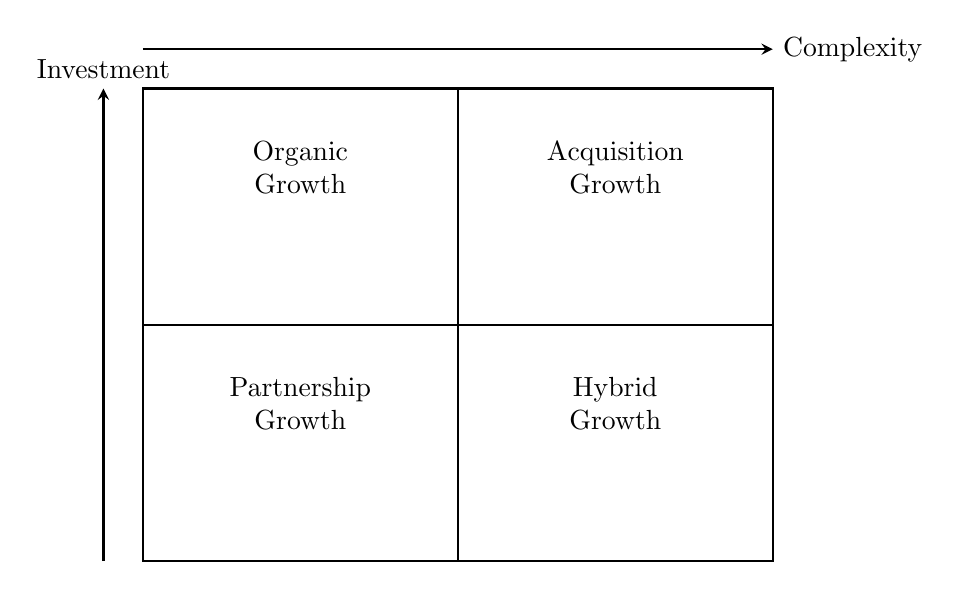
\begin{tikzpicture}[
        box/.style={draw, minimum size=1cm, text width=2cm, align=center}
    ]
        % Growth model matrix
        \draw[thick] (0,0) rectangle (8,6);
        \draw[thick] (4,0) -- (4,6);
        \draw[thick] (0,3) -- (8,3);

        % Labels with better formatting
        \node[text width=3cm, align=center] at (2,5) {Organic\\Growth};
        \node[text width=3cm, align=center] at (6,5) {Acquisition\\Growth};
        \node[text width=3cm, align=center] at (2,2) {Partnership\\Growth};
        \node[text width=3cm, align=center] at (6,2) {Hybrid\\Growth};

        % Arrows indicating complexity
        \draw[-stealth, thick] (0,6.5) -- (8,6.5) node[right] {Complexity};
        \draw[-stealth, thick] (-0.5,0) -- (-0.5,6) node[above] {Investment};
    \end{tikzpicture}
    \caption{Growth Strategy Matrix}
    \label{fig:growth-matrix}
\end{figure}

\subsection{Expansion Timeline Planning}
\begin{center}
\begin{tabularx}{\textwidth}{>{\raggedright\arraybackslash}X >{\centering\arraybackslash}X >{\raggedright\arraybackslash}X >{\raggedright\arraybackslash}X}
    \toprule
    \textbf{Phase} & \textbf{Duration} & \textbf{Focus} & \textbf{Key Metrics} \\
    \midrule
    Foundation & 6 months & Core operations & Stability \\
    Growth & 12 months & Market expansion & Revenue \\
    Scale & 18 months & Regional presence & Market share \\
    Optimize & Ongoing & Efficiency & Profitability \\
    \bottomrule
\end{tabularx}
\end{center}

\FloatBarrier
\section{Team Building and Management}

\subsection{Organizational Structure Evolution}
\begin{figure}[htbp]
    \centering
    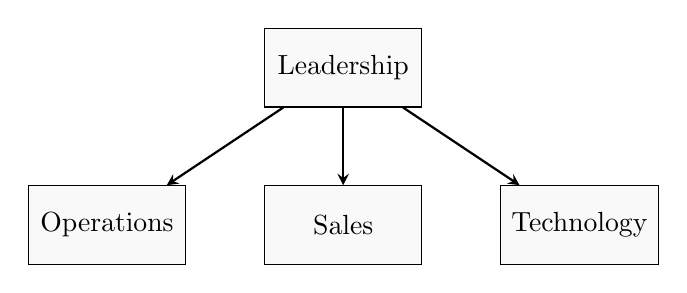
\begin{tikzpicture}[
        node distance=2cm,
        box/.style={draw, minimum width=2cm, minimum height=1cm, align=center, fill=gray!5},
        arrow/.style={-stealth, thick}
    ]
        % Org structure evolution
        \node[box] (ceo) at (0,0) {Leadership};
        \node[box] (ops) at (-3,-2) {Operations};
        \node[box] (sales) at (0,-2) {Sales};
        \node[box] (tech) at (3,-2) {Technology};

        \draw[arrow] (ceo) -- (ops);
        \draw[arrow] (ceo) -- (sales);
        \draw[arrow] (ceo) -- (tech);
    \end{tikzpicture}
    \caption{Scalable Organization Structure}
    \label{fig:org-structure}
\end{figure}

\FloatBarrier
\section{Regional Growth Pathways}

% UK Region
\begin{regionalbox}{United Kingdom}
\textbf{Financial Services Scaling}
\begin{itemize}
    \item Regulatory capacity building
    \item Service portfolio expansion
    \item Market segment penetration
    \item Cross-border operations
\end{itemize}
\end{regionalbox}

\subsection{UK Market Development}
\begin{figure}[htbp]
    \centering
    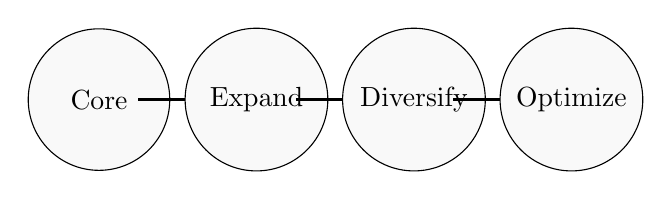
\begin{tikzpicture}[
        node distance=2cm,
        phase/.style={draw, circle, text width=1.5cm, align=center, fill=gray!5},
        arrow/.style={-stealth, thick}
    ]
        % Market development stages
        \foreach \x/\label in {0/Core,2/Expand,4/Diversify,6/Optimize}
        {
            \node[phase] at (\x,0) {\label};
            \ifnum\x<6
                \draw[arrow] (\x+0.5,0) -- (\x+1.5,0);
            \fi
        }
    \end{tikzpicture}
    \caption{Financial Services Growth Path}
    \label{fig:uk-growth}
\end{figure}

% US Region
\begin{regionalbox}{United States}
\textbf{Tech Platform Expansion}
\begin{itemize}
    \item Product feature scaling
    \item User base growth
    \item Infrastructure expansion
    \item Market penetration
\end{itemize}
\end{regionalbox}

\subsection{US Growth Metrics}
\begin{center}
\begin{tabularx}{\textwidth}{>{\raggedright\arraybackslash}X >{\centering\arraybackslash}X >{\centering\arraybackslash}X}
    \toprule
    \textbf{Metric} & \textbf{Target} & \textbf{Timeline} \\
    \midrule
    User Growth & 200\% YoY & 12 months \\
    Revenue Growth & 150\% YoY & 12 months \\
    Market Share & 15\% & 24 months \\
    \bottomrule
\end{tabularx}
\end{center}

% UAE Region
\begin{regionalbox}{UAE}
\textbf{Trade Network Development}
\begin{itemize}
    \item Supply chain expansion
    \item Market coverage growth
    \item Partner network development
    \item Operational capacity
\end{itemize}

\subsection{UAE Trade Growth Framework}
\begin{tcolorbox}[colback=white,colframe=primary,title=\textbf{Growth Components}]
\begin{enumerate}
    \item Geographic expansion
    \item Product line growth
    \item Service enhancement
    \item Partner integration
    \item Market penetration
\end{enumerate}
\end{tcolorbox}
\end{regionalbox}

% Canada Region
\begin{regionalbox}{Canada}
\textbf{Market Penetration Strategy}
\begin{itemize}
    \item Sector expansion
    \item Technology adoption
    \item Regulatory compliance
    \item Market positioning
\end{itemize}
\end{regionalbox}

\subsection{Canadian Market Growth}
\begin{center}
\begin{tabularx}{\textwidth}{>{\raggedright\arraybackslash}X >{\raggedright\arraybackslash}X >{\centering\arraybackslash}X}
    \toprule
    \textbf{Sector} & \textbf{Growth Strategy} & \textbf{Timeline} \\
    \midrule
    AgriTech & Market expansion & 18 months \\
    CleanTech & Partnership growth & 24 months \\
    Education & Service expansion & 12 months \\
    \bottomrule
\end{tabularx}
\end{center}

\FloatBarrier
\section{Quality Control Systems}

\subsection{Growth Quality Framework}
\begin{figure}[htbp]
    \centering
    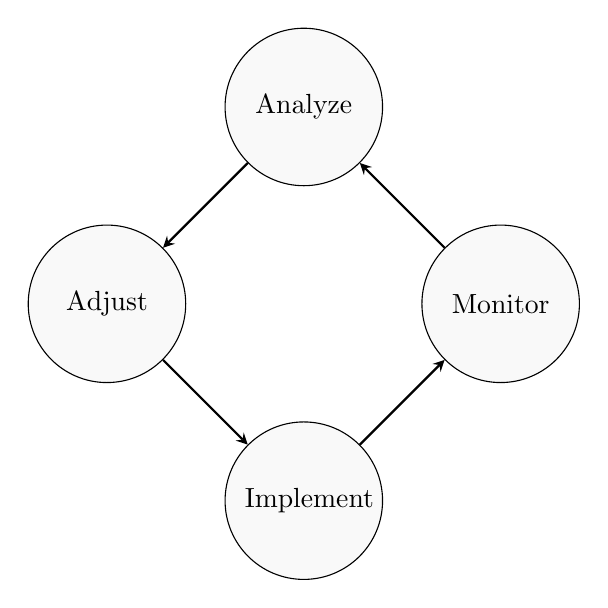
\begin{tikzpicture}[
        node distance=3cm,
        phase/.style={draw, circle, minimum size=2cm, text width=1.5cm, align=center, fill=gray!5},
        arrow/.style={-stealth, thick, bend left=15}
    ]
        % Quality control cycle with improved styling
        \foreach \angle/\label in {
            0/Monitor,
            90/Analyze,
            180/Adjust,
            270/Implement
        } {
            \node[phase] (phase-\angle) at (\angle:2.5) {\label};
        }

        % Connect phases with curved arrows
        \draw[arrow] (phase-0) -- (phase-90);
        \draw[arrow] (phase-90) -- (phase-180);
        \draw[arrow] (phase-180) -- (phase-270);
        \draw[arrow] (phase-270) -- (phase-0);
    \end{tikzpicture}
    \caption{Growth Quality Management}
    \label{fig:quality-management}
\end{figure}

\section{Performance Metrics}

\begin{tcolorbox}[colback=white,colframe=primarydark,title=\textbf{Growth KPIs}]
\begin{itemize}
    \item Revenue Growth Rate
    \item Market Share
    \item Customer Acquisition Cost
    \item Customer Lifetime Value
    \item Operational Efficiency
\end{itemize}
\end{tcolorbox}

\begin{communitybox}
Access growth and scaling resources on the Africa Growth Circle:
\begin{itemize}
    \item Growth strategy templates
    \item Scaling case studies
    \item Expert mentorship
    \item Peer networking
    \item Market intelligence
\end{itemize}
Visit circle.counseal.com for growth support.
\end{communitybox}

\begin{workshopbox}
\textbf{Chapter 9 Growth Planning Workshop}

1. Growth Strategy Development
\begin{itemize}
    \item Growth model selected: \_\_\_\_\_\_\_\_\_
    \item Target metrics: \_\_\_\_\_\_\_\_\_
    \item Resource requirements: \_\_\_\_\_\_\_\_\_
\end{itemize}

2. Team Scaling Plan
\begin{itemize}
    \item Organizational structure: \_\_\_\_\_\_\_\_\_
    \item Key positions: \_\_\_\_\_\_\_\_\_
    \item Timeline: \_\_\_\_\_\_\_\_\_
\end{itemize}

3. Market Expansion
\begin{itemize}
    \item Target markets: \_\_\_\_\_\_\_\_\_
    \item Entry strategy: \_\_\_\_\_\_\_\_\_
    \item Growth milestones: \_\_\_\_\_\_\_\_\_
\end{itemize}

Download growth planning templates from the Africa Growth Circle platform.
\end{workshopbox}

\begin{importantbox}
In Chapter 10, we'll explore strategies for future-proofing your business and staying ahead of market trends.
\end{importantbox}